\documentclass[t, aspectratio=169]{beamer}
\usepackage[utf8]{vietnam}
\usepackage{amsthm,amsmath,amssymb}
\usepackage{lmodern}
\usepackage{booktabs}
\usepackage{colortbl}

% --- CẤU HÌNH LỀ (giống Slide_HUST.tex mẫu) ---
\def\slideContentLeftMargin{0.5cm}
\def\slideContentRightMargin{1cm}
\def\hustHeaderHeight{1cm}
\def\slideContentBotMargin{3.5cm}

\usepackage[red, 169]{beamerthemeHUST}

% Thêm graphicspath cho figures luận văn
\graphicspath{{images/}{../report_latex/figures/}}

% --- TITLE PAGE ---
\renewcommand{\titlePageTitleX}{-0.5cm}
\renewcommand{\titlePageTitleY}{-0.5cm}
\renewcommand{\hustTitleAlign}{\alignLeft}
\renewcommand{\hustSubtitleAlign}{\alignLeft}
\renewcommand{\hustAuthorAlign}{\alignLeft}
\renewcommand{\hustInstAlign}{\alignLeft}

% Title ngắn → \Huge không quá to; subtitle mang tên đề tài → \Large vừa
\title{ĐỒ ÁN TỐT NGHIỆP}
\subtitle{Đề xuất mô hình CDDFuse-AG\\cho tổng hợp ảnh y tế đa phương thức}
\author{Đỗ Trung Kiên --- 20224869}
\institute{GVHD: TS. Phạm Đăng Hải · PGS. TS. Phạm Văn Hải}

\begin{document}

\hustintropage{}
\hustsectionpage{}

\husttitlepage

\begin{frame}[allowframebreaks]{Nội dung trình bày}
    \tableofcontents[hideallsubsections]
\end{frame}

\resetPageCount
\showPageNumber

% =================================================================
\section{Giới thiệu và bài toán (Introduction)}
% =================================================================
\useStyleHustFull
\useThinBar

\begin{frame}{Bài toán tổng hợp ảnh y tế đa phương thức}
    \begin{columns}[T]
        \begin{column}{0.50\textwidth}
            \textbf{Mỗi phương thức ảnh có ưu điểm riêng:}
            \begin{itemize}\itemsep1pt
                \item \textbf{MRI}: Độ phân giải cao về mô mềm
                \item \textbf{CT}: Rõ cấu trúc xương
                \item \textbf{PET/SPECT}: Thông tin chức năng, trao đổi chất
            \end{itemize}
            \vspace{0.15em}
            \textbf{MIF} kết hợp hai phương thức thành \alert{một ảnh duy nhất} --- hỗ trợ chẩn đoán nhanh và chính xác hơn.
            \vspace{0.15em}

            \textbf{Thách thức:} Không tồn tại ảnh chuẩn $\Rightarrow$ hàm mất mát không giám sát.
        \end{column}
        \begin{column}{0.46\textwidth}
            \begin{figure}
                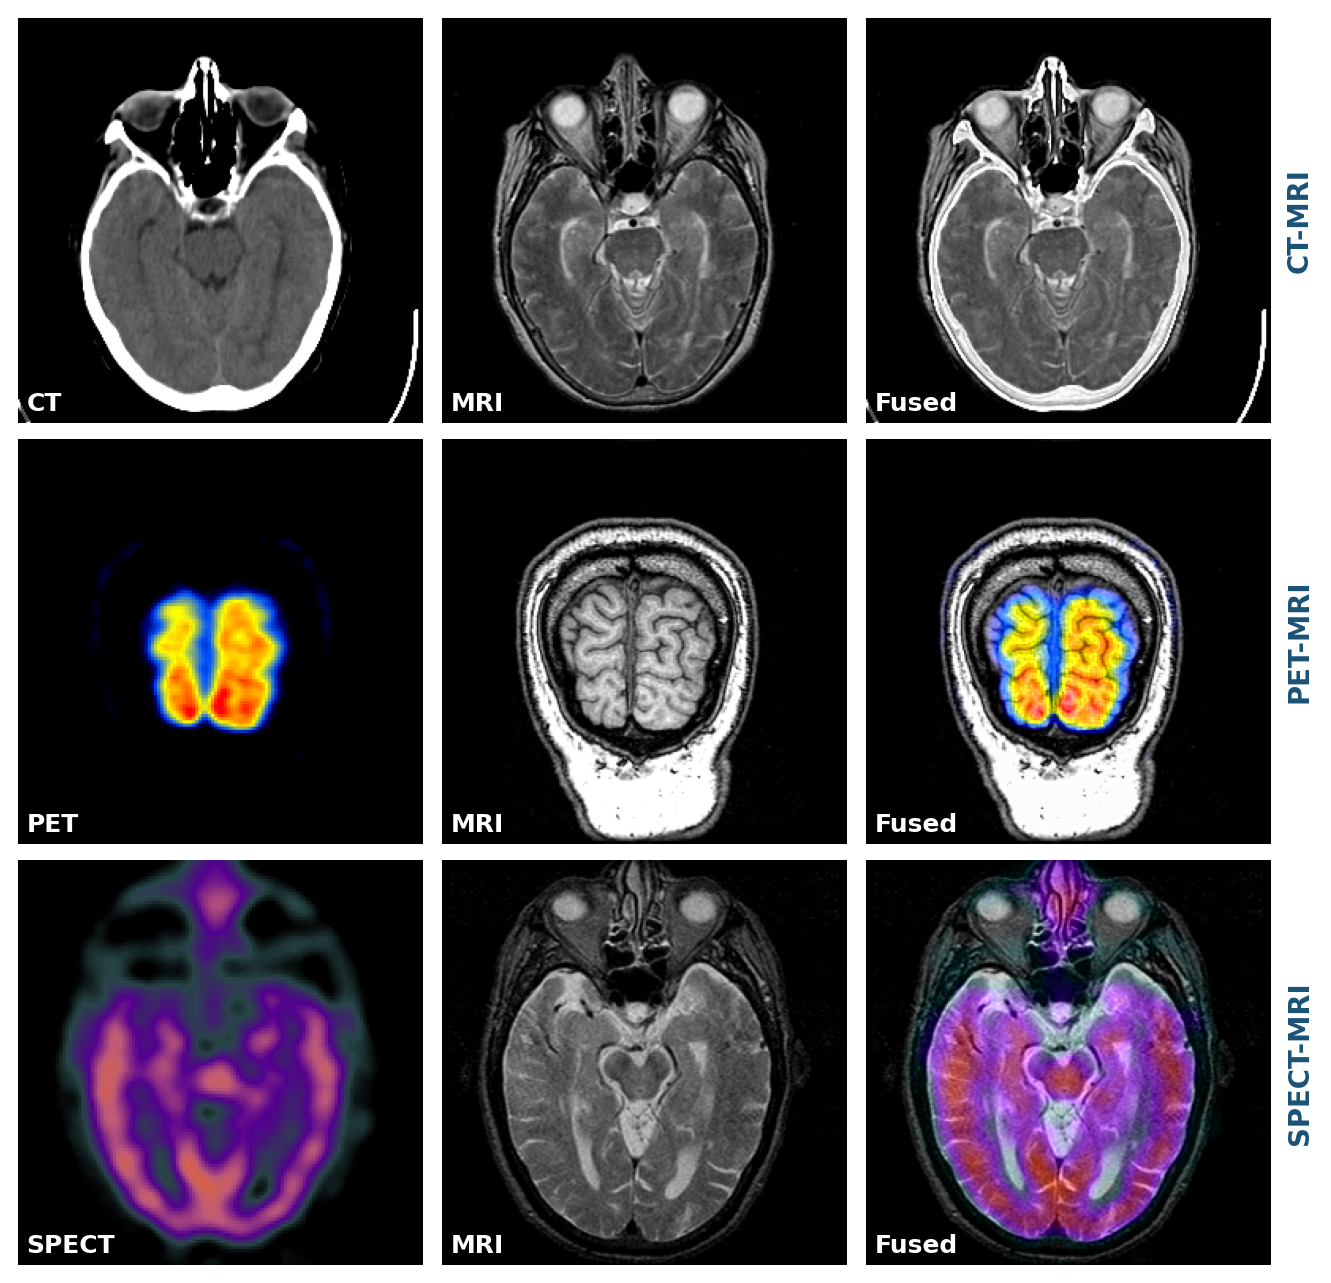
\includegraphics[width=\textwidth,height=0.48\textheight,keepaspectratio]{fig1_mif_examples.png}
                \caption{\small CT-MRI, PET-MRI, SPECT-MRI trên Harvard MIF.}
            \end{figure}
        \end{column}
    \end{columns}
\end{frame}

\begin{frame}{Tập dữ liệu và thiết lập thực nghiệm}
    \begin{columns}[T]
        \begin{column}{0.50\textwidth}
            \textbf{Harvard Medical Image Fusion Dataset:}
            \begin{itemize}\itemsep2pt\small
                \item \textbf{738 cặp train} + \textbf{72 cặp test} (24 CT + 24 PET + 24 SPECT ghép với MRI)
                \item 5 bệnh nhân $\times$ ~15 lát cắt mỗi bệnh nhân
                \item Ảnh não người (brain MRI) --- độ phân giải $256\times256$
            \end{itemize}
            \vspace{0.4em}
            \begin{block}{\small Chỉ số đánh giá (8 nhóm)}
                \small
                \begin{tabular}{ll}
                    SSIM, PSNR & cấu trúc tổng thể \\
                    SF, AG, EI & cạnh / tần số cao \\
                    Qabf, QM   & truyền thông tin \\
                    MI, QMI    & thông tin chung \\
                \end{tabular}
            \end{block}
        \end{column}
        \begin{column}{0.46\textwidth}
            \begin{figure}
                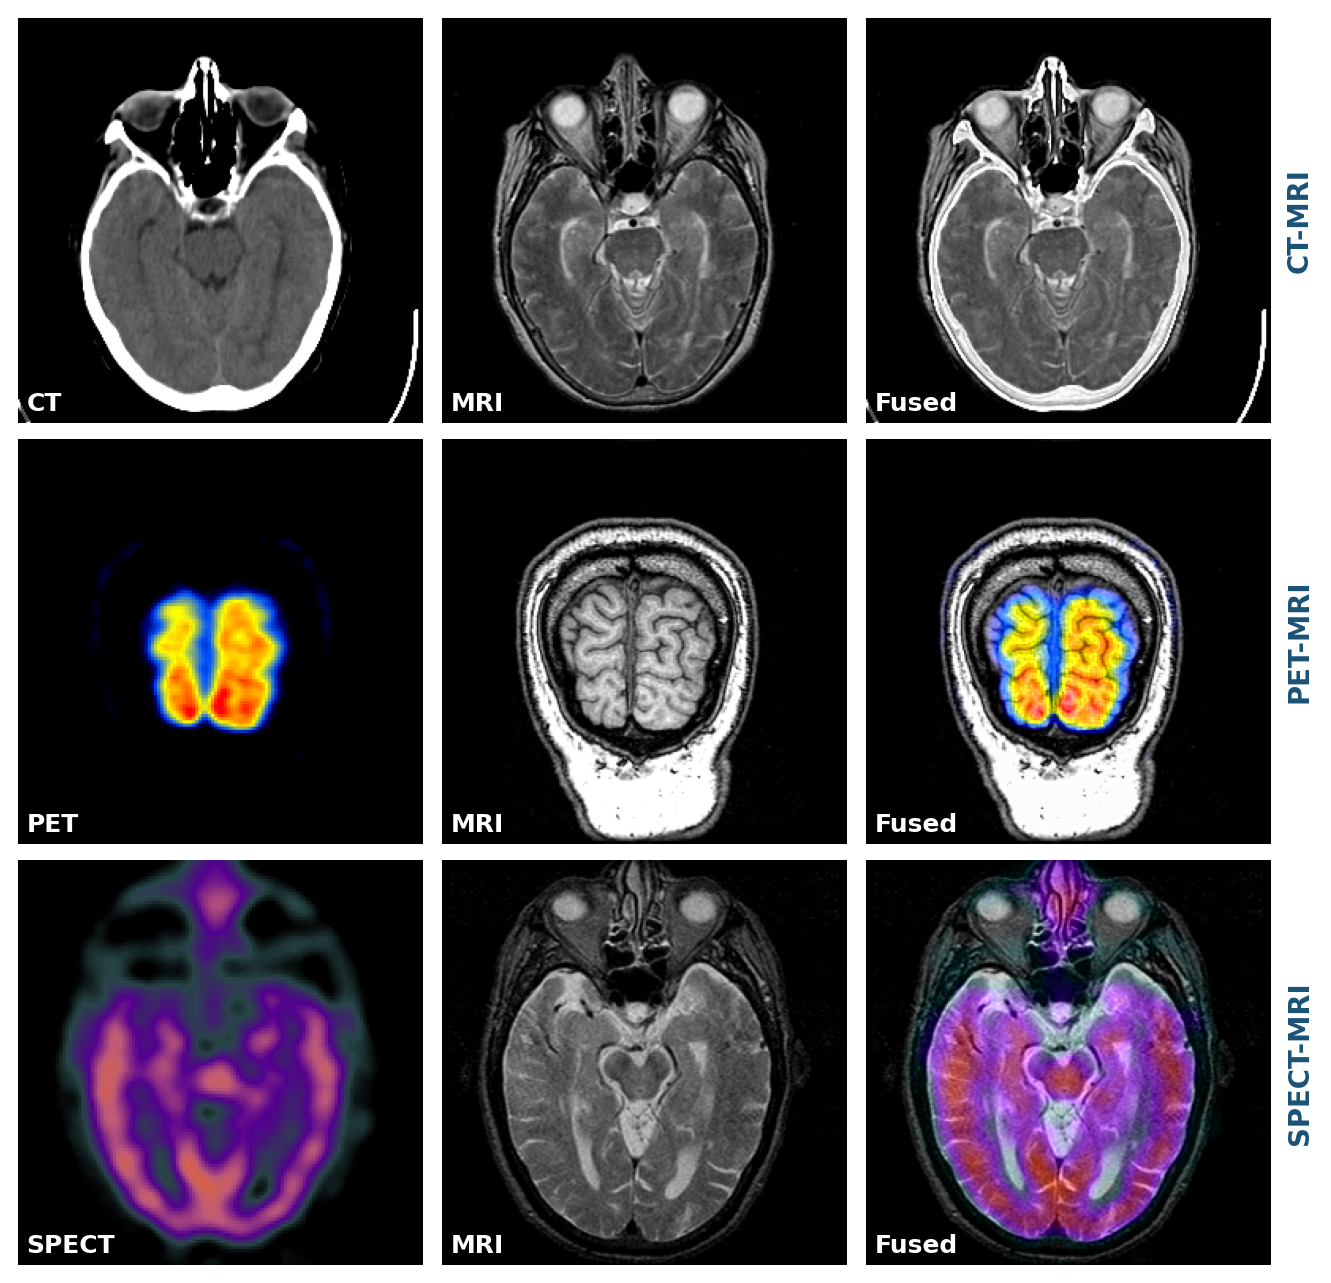
\includegraphics[width=\textwidth,height=0.52\textheight,keepaspectratio]{fig1_mif_examples.png}
                \caption{\small Mẫu ảnh Harvard MIF: MRI (trái), CT/PET/SPECT (phải).}
            \end{figure}
        \end{column}
    \end{columns}
\end{frame}

\begin{frame}{Tại sao CDDFuse? Và hạn chế nào cần cải tiến?}
    \begin{columns}[T]
        \begin{column}{0.52\textwidth}
            \textbf{CDDFuse} (Zhao et al., CVPR 2023) --- \#2/22 SOTA:
            \begin{itemize}
                \item Dual-branch: tách nhánh \textbf{Base} (tần số thấp) và \textbf{Detail} (tần số cao)
                \item Restormer Encoder + Invertible Neural Network
                \item Huấn luyện không giám sát trên dữ liệu y tế
            \end{itemize}
            \vspace{0.3em}
            \textbf{Hạn chế:} Cả hai nhánh dùng chung \alert{phép cộng đơn giản}:
            \[ f_F = f_V + f_I \]
            Không khai thác \textbf{bản chất khác nhau} giữa tần số thấp và tần số cao.
        \end{column}
        \begin{column}{0.44\textwidth}
            \begin{alertblock}{Điểm can thiệp}
                Chỉ thay thế \textbf{Fusion Layer}, giữ nguyên Encoder--Decoder pretrained.\\[4pt]
                $\Rightarrow$ So sánh công bằng, tốn ít tài nguyên.
            \end{alertblock}
            \vspace{0.5em}
            \begin{block}{Câu hỏi nghiên cứu}
                \small Dùng quy tắc \textbf{khác nhau cho từng nhánh} (bất đối xứng) có cải thiện chất lượng tổng hợp không?
            \end{block}
        \end{column}
    \end{columns}
\end{frame}

% =================================================================
\section{Các nghiên cứu liên quan (Related Work)}
% =================================================================
\useStyleHustFull
\useThinBar

\begin{frame}{Tiến trình nghiên cứu tổng hợp ảnh y tế}
    \begin{columns}[T]
        \begin{column}{0.48\textwidth}
            \textbf{Phương pháp truyền thống:}
            \begin{itemize}\itemsep1pt\small
                \item Laplacian pyramid, Wavelet --- phân rã đa tỉ lệ, không cần học
                \item Hạn chế: tham số thủ công, không thích nghi với dữ liệu
            \end{itemize}
            \vspace{0.3em}
            \textbf{CNN và học biểu diễn:}
            \begin{itemize}\itemsep1pt\small
                \item DenseFuse, NestFuse, RFN-Nest --- encoder học đặc trưng
                \item Fusion rule vẫn cố định (L1, Weighted Avg)
            \end{itemize}
            \vspace{0.3em}
            \textbf{GAN:}
            \begin{itemize}\itemsep1pt\small
                \item FusionGAN --- bảo toàn chi tiết qua adversarial loss
                \item Huấn luyện không ổn định, dễ mode collapse
            \end{itemize}
        \end{column}
        \begin{column}{0.48\textwidth}
            \textbf{Transformer và mô hình sinh:}
            \begin{itemize}\itemsep1pt\small
                \item SwinFusion, CDDFuse, DDFM, TUFusion --- attention toàn cục
                \item DDFM dùng diffusion model, chất lượng cao nhưng rất chậm
            \end{itemize}
            \vspace{0.5em}
            \begin{alertblock}{Khoảng trống nghiên cứu}
                \small Hầu hết phương pháp dùng \textbf{cùng quy tắc} cho cả nhánh Base (tần số thấp) và Detail (tần số cao) --- không khai thác bản chất khác nhau của hai nhánh.\\[4pt]
                $\Rightarrow$ CDDFuse-AG đề xuất \textbf{quy tắc bất đối xứng}.
            \end{alertblock}
        \end{column}
    \end{columns}
\end{frame}

% =================================================================
\section{Phương pháp đề xuất (Proposed Method)}
% =================================================================
\useStyleLogoOnly
\useThickBar

\begin{frame}{Nguyên lý thiết kế bất đối xứng}
    \begin{columns}[T]
        \begin{column}{0.48\textwidth}
            \begin{block}{Nhánh Base (tần số thấp)}
                Mang thông tin cấu trúc toàn cục.\\
                Hai modality có \textbf{tương quan cao}.\\
                $\Rightarrow$ Cần \textbf{trung bình hóa} (averaging).
            \end{block}
            \vspace{0.4em}
            \begin{block}{Nhánh Detail (tần số cao)}
                Mang cạnh, texture đặc thù từng modality.\\
                Thông tin \textbf{bổ trợ nhau}.\\
                $\Rightarrow$ Cần \textbf{lựa chọn cục bộ} (activity-based selection).
            \end{block}
            \vspace{0.4em}
            \small Phép cộng Sum áp dụng \emph{cùng chiến lược} cho cả hai --- \alert{không tối ưu}.
        \end{column}
        \begin{column}{0.48\textwidth}
            \begin{figure}
                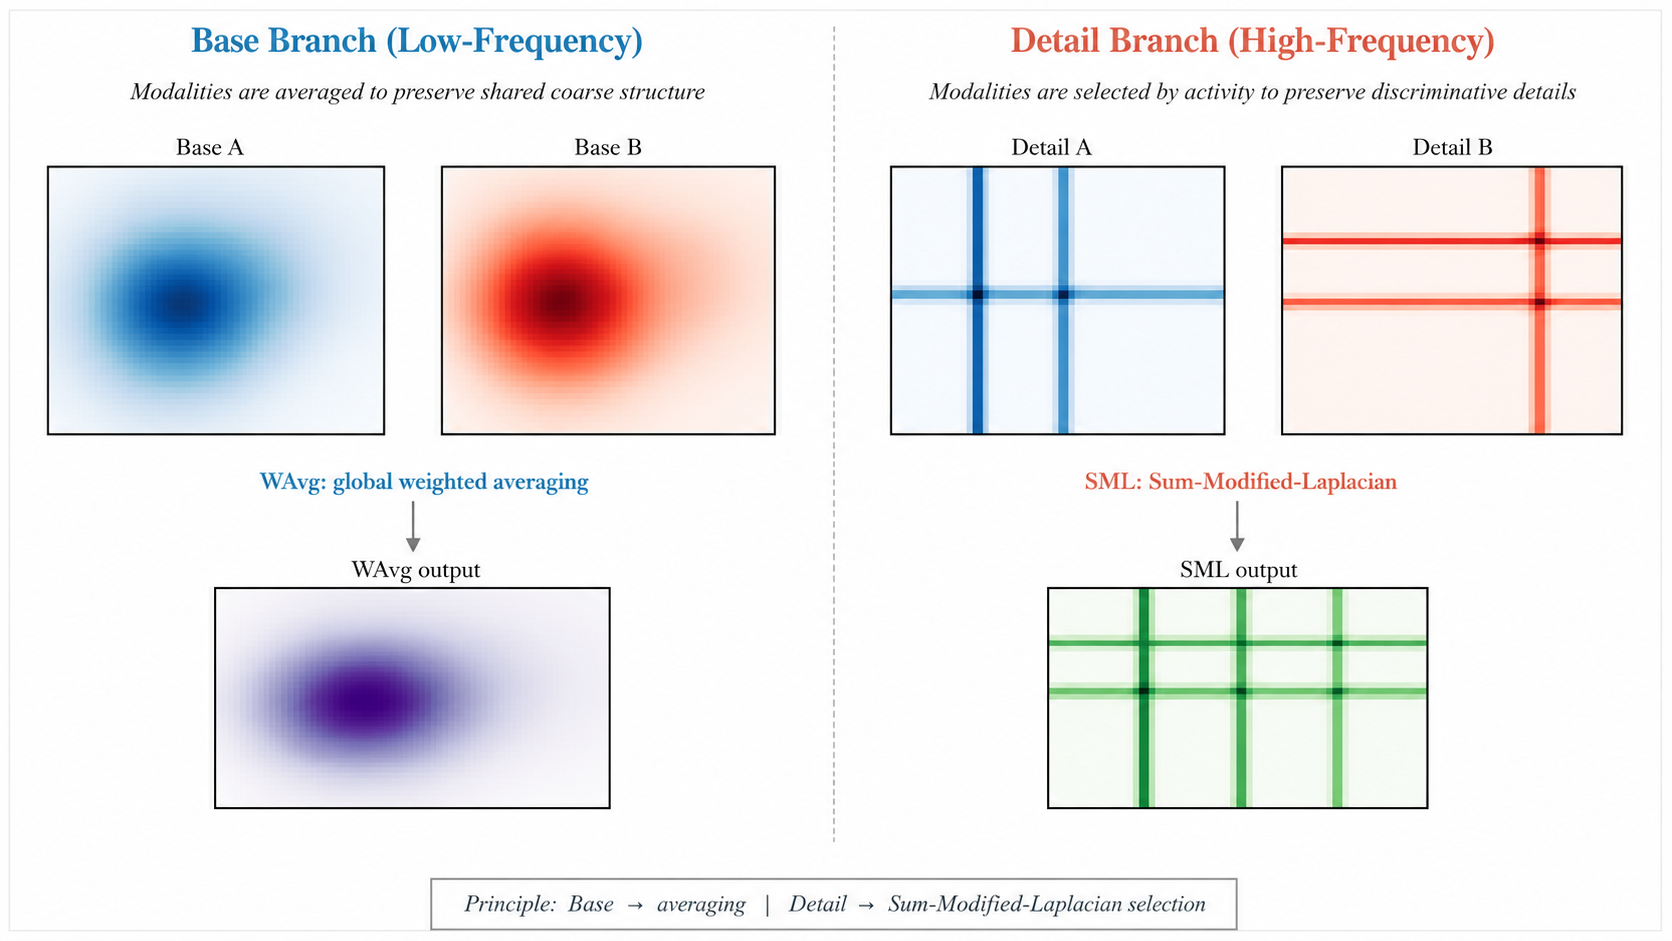
\includegraphics[width=\textwidth]{fig_asymmetric_principle.png}
                \caption{\small WAvg phù hợp Base (đồng thuận); SML phù hợp Detail (bổ trợ).}
            \end{figure}
        \end{column}
    \end{columns}
\end{frame}

\begin{frame}{Quy tắc Base: Weighted Average Scalar (WAvg)}
    \begin{columns}[T]
        \begin{column}{0.50\textwidth}
            Trung bình có trọng số với \textbf{1 scalar học được} $\theta$:
            \begin{align}
                \alpha &= \sigma(\theta), \quad \theta \in \mathbb{R} \\[4pt]
                R_{\mathrm{WAvg}}(a,b) &= 2\bigl(\alpha \cdot a + (1-\alpha) \cdot b\bigr)
            \end{align}
            \vspace{0.2em}
            \begin{itemize}
                \item Chỉ \textbf{1 tham số học} --- tránh overfitting
                \item Tự học tỉ lệ $\alpha$ tối ưu cho từng modality
                \item Khởi tạo $\theta=0$ ($\alpha=0.5$) --- ổn định khi chuyển pha
            \end{itemize}
        \end{column}
        \begin{column}{0.46\textwidth}
            \begin{figure}
                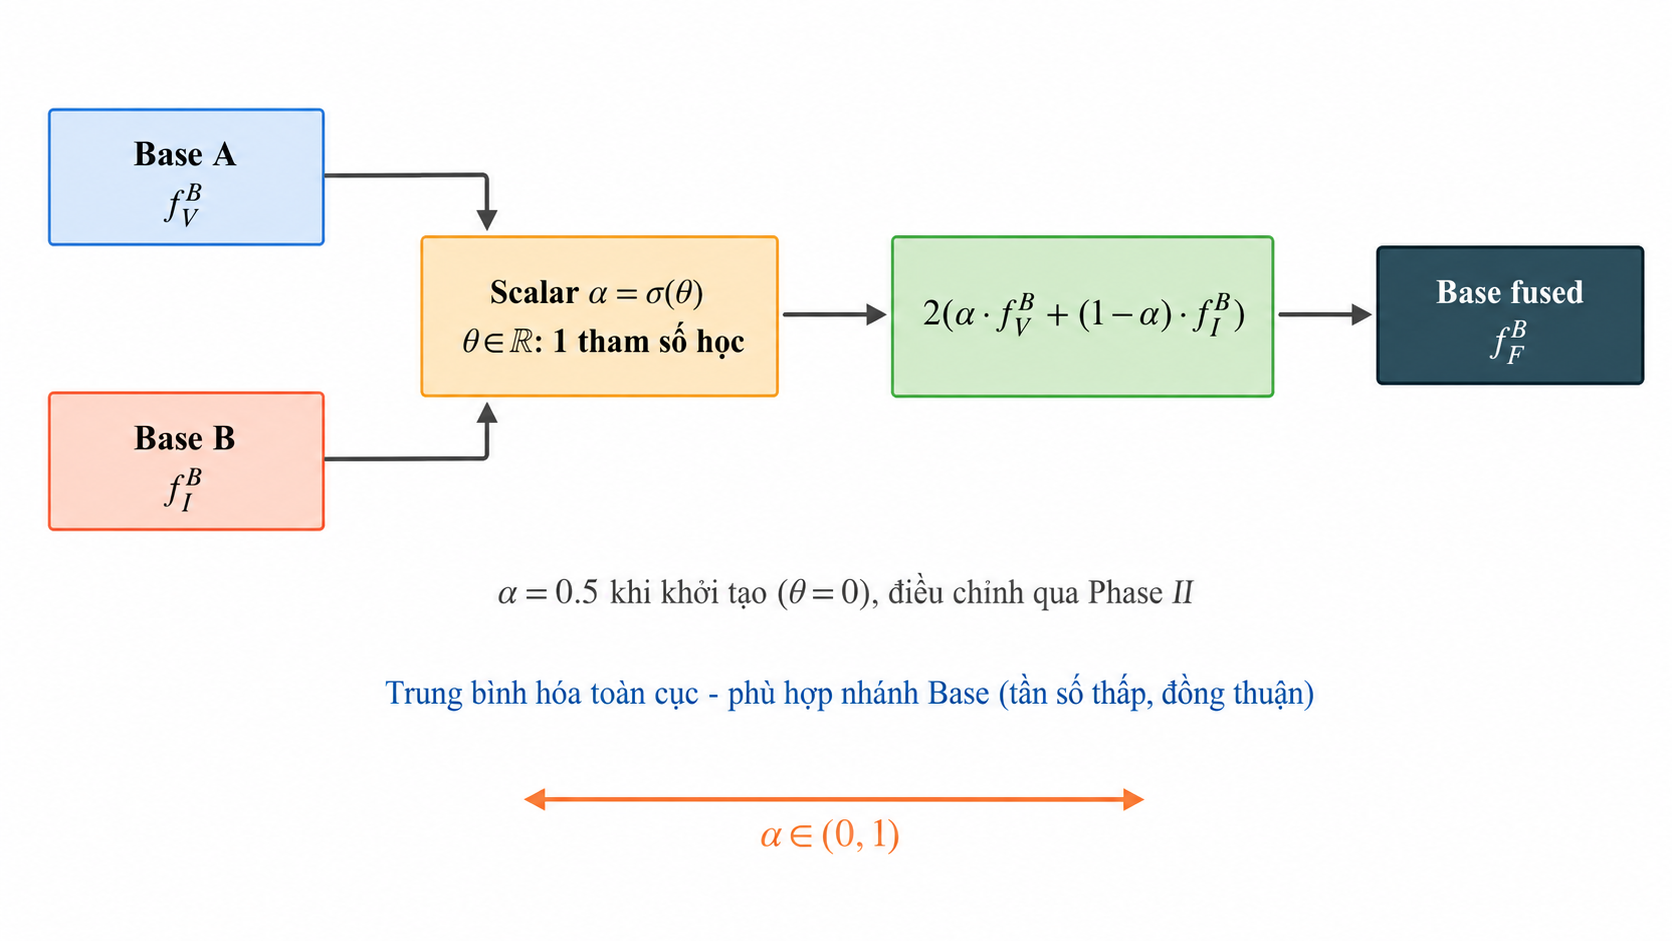
\includegraphics[width=\textwidth]{fig_rule_wavg.png}
                \caption{\small WAvg: hai Feature Map Base kết hợp bằng scalar $\alpha$.}
            \end{figure}
        \end{column}
    \end{columns}
\end{frame}

\begin{frame}{Quy tắc Detail: Sum-Modified-Laplacian (SML)}
    \begin{columns}[T]
        \begin{column}{0.50\textwidth}
            Tại mỗi vị trí, chọn modality có cạnh \textbf{sắc nét hơn}:
            \begin{align}
                \mathrm{ML}_{ij} &= |2f_{ij}{-}f_{i-1,j}{-}f_{i+1,j}| + |2f_{ij}{-}f_{i,j-1}{-}f_{i,j+1}| \\
                w_a &= \tfrac{\mathrm{SML}(a)}{\mathrm{SML}(a)+\mathrm{SML}(b)+\varepsilon} \\
                R_{\mathrm{SML}} &= 2\bigl(w_a \odot a + (1-w_a) \odot b\bigr)
            \end{align}
            \begin{itemize}
                \item \textbf{Không tham số học} --- tổng quát hóa tốt
                \item Lựa chọn \textbf{theo từng vị trí} (spatially adaptive)
            \end{itemize}
        \end{column}
        \begin{column}{0.46\textwidth}
            \begin{figure}
                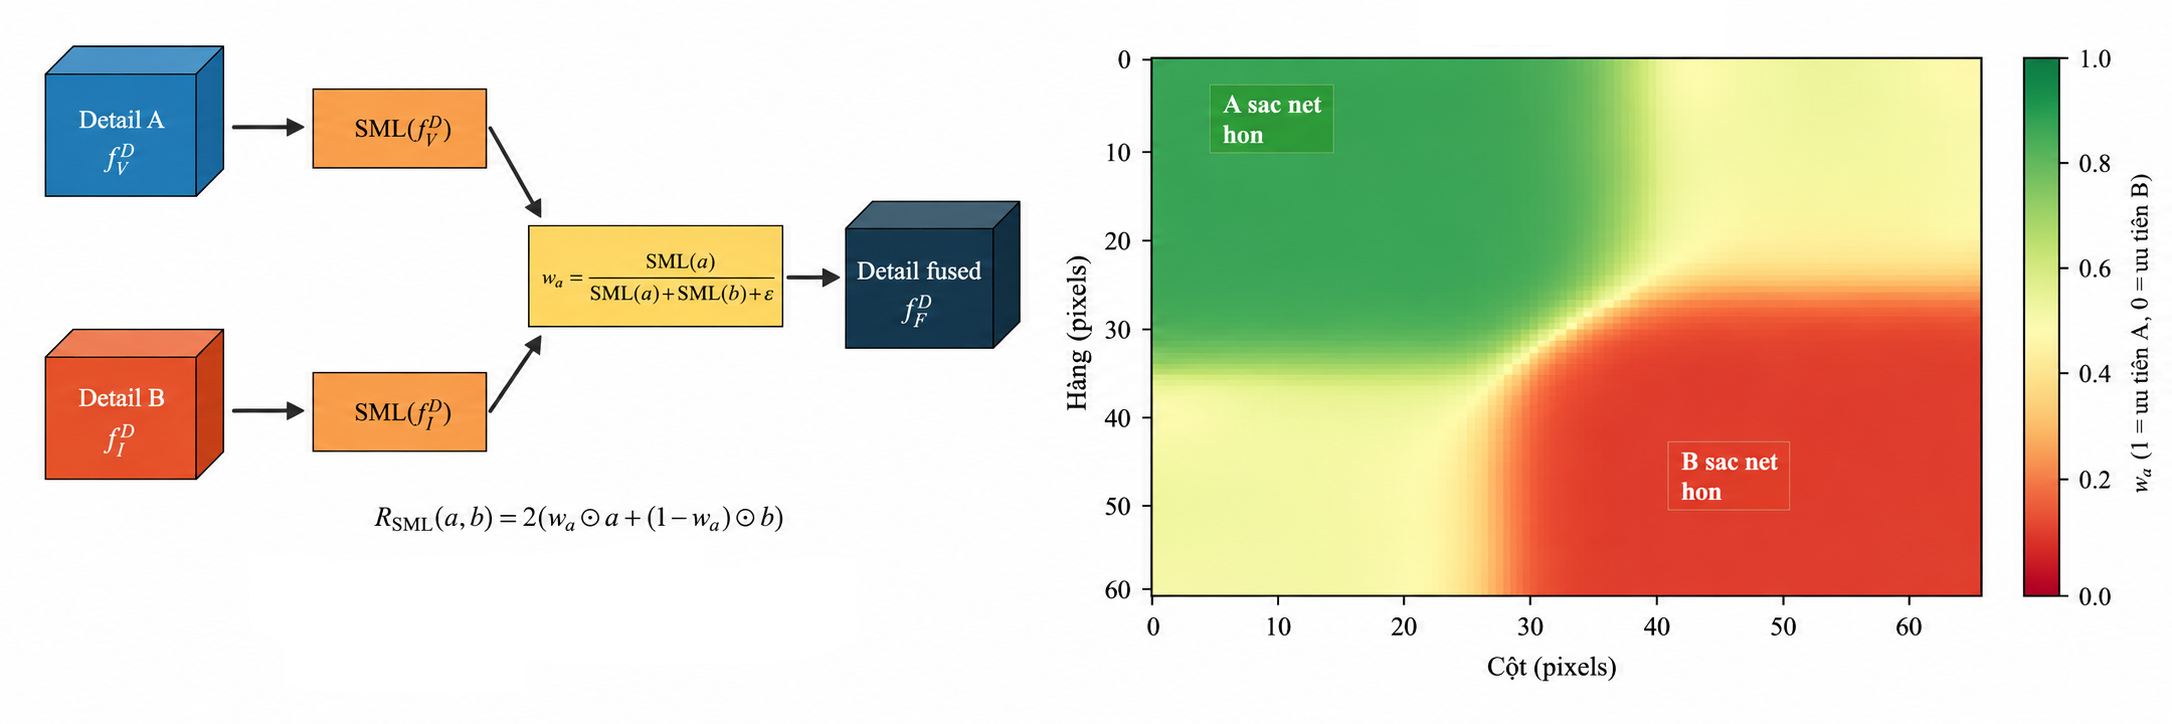
\includegraphics[width=\textwidth]{fig_rule_sml.png}
                \caption{\small Xanh = ưu tiên Detail A; Đỏ = ưu tiên Detail B.}
            \end{figure}
        \end{column}
    \end{columns}
\end{frame}

\begin{frame}{Tại sao Sum làm mờ nhánh Detail?}
    \begin{columns}[T]
        \begin{column}{0.52\textwidth}
            \textbf{Phân tích tần số: phép cộng Sum trên Detail}\\[4pt]
            Khi hai tín hiệu cùng tần số $f$ nhưng lệch pha $\phi$:
            \[
              A\cos(2\pi f t) + A\cos(2\pi f t + \phi) = 2A\cos\!\tfrac{\phi}{2}\cdot\cos\!\bigl(2\pi f t + \tfrac{\phi}{2}\bigr)
            \]
            \vspace{-0.2em}
            \begin{itemize}\itemsep1pt\small
                \item Biên độ bị nhân bởi $\cos(\phi/2) \leq 1$
                \item Khi CT và MRI có cạnh \textbf{lệch vị trí} ($\phi \neq 0$): Sum làm \alert{suy giảm biên độ cạnh}
                \item Kết quả: viền xương/mô mềm bị làm mờ trong ảnh tổng hợp
            \end{itemize}
            \vspace{0.4em}
            \textbf{SML khắc phục:} tại mỗi pixel, \emph{chọn} modality có Laplacian lớn hơn thay vì cộng --- không làm suy giảm biên độ.
        \end{column}
        \begin{column}{0.44\textwidth}
            \begin{alertblock}{Minh họa trực quan}
                \small
                \begin{tabular}{lcc}
                    & \textbf{CT cạnh} & \textbf{MRI cạnh} \\
                    \midrule
                    Vị trí & 40px & 42px \\
                    Sum & \multicolumn{2}{c}{\alert{biên độ giảm ~$\cos(2°)$}} \\
                    SML & \multicolumn{2}{c}{\textbf{chọn CT, biên độ gốc}} \\
                \end{tabular}
            \end{alertblock}
            \vspace{0.4em}
            \begin{block}{\small Kết luận}
                \small Nhánh Detail cần \textbf{lựa chọn cục bộ}, không trung bình --- đây là lý do SML phù hợp hơn Sum về mặt lý thuyết.
            \end{block}
        \end{column}
    \end{columns}
\end{frame}

\begin{frame}{Chiến lược huấn luyện (Training Protocol)}
    \begin{columns}[T]
        \begin{column}{0.52\textwidth}
            \textbf{Phase I --- Reconstruction (từ CDDFuse pretrained):}
            \begin{itemize}\itemsep2pt\small
                \item Encoder và Decoder học phân rã ảnh thành Base + Detail
                \item Loss: $\mathcal{L} = \mathcal{L}_\text{pixel} + \lambda_1\mathcal{L}_\text{SSIM} + \lambda_2\mathcal{L}_\text{feature}$
                \item \textbf{Giữ nguyên} weights Phase I của CDDFuse gốc
            \end{itemize}
            \vspace{0.5em}
            \textbf{Phase II --- Fusion Fine-tune (CDDFuse-AG):}
            \begin{itemize}\itemsep2pt\small
                \item Chỉ cập nhật \textbf{Fusion Layer} (WAvg + SML)
                \item $\theta$ (scalar WAvg) khởi tạo bằng 0 ($\alpha = 0.5$)
                \item 100 epochs, Adam, lr = $1\times10^{-4}$
                \item Loss bổ sung gradient term để hướng đến SF/AG cao hơn
            \end{itemize}
        \end{column}
        \begin{column}{0.44\textwidth}
            \begin{block}{\small Lợi thế của chiến lược này}
                \small
                \begin{itemize}\itemsep3pt
                    \item Encoder/Decoder \textbf{không cần train lại} --- tiết kiệm 95\% thời gian
                    \item So sánh \textbf{công bằng} với CDDFuse (cùng backbone)
                    \item Chỉ thêm \textbf{4.161 tham số} ($\sim$0.35\%)
                    \item Dễ dàng mở rộng sang quy tắc fusion mới
                \end{itemize}
            \end{block}
            \vspace{0.3em}
            \begin{alertblock}{\small Phần được thay đổi}
                \centering\small \texttt{BaseFuseLayer}: Sum $\to$ \textbf{WAvg}\\
                \texttt{DetailFuseLayer}: Sum $\to$ \textbf{SML}
            \end{alertblock}
        \end{column}
    \end{columns}
\end{frame}

\begin{frame}{Kiến trúc CDDFuse-AG}
    \begin{columns}[T]
        \begin{column}{0.35\textwidth}
            \textbf{Thay đổi duy nhất:}
            \begin{itemize}
                \item Base: Sum $\rightarrow$ \textbf{WAvg}
                \item Detail: Sum $\rightarrow$ \textbf{SML}
            \end{itemize}
            \vspace{0.5em}
            \begin{block}{Tham số bổ sung}
                \small
                \begin{tabular}{lr}
                    \toprule
                    WAvg ($\theta$)     & 1     \\
                    SML refine Conv     & 4,160 \\
                    \midrule
                    \textbf{Tổng mới}   & \textbf{4,161} \\
                    \bottomrule
                \end{tabular}\\[4pt]
                \footnotesize ($\sim$0.35\% của 1,188,272 params CDDFuse)
            \end{block}
        \end{column}
        \begin{column}{0.61\textwidth}
            \begin{figure}
                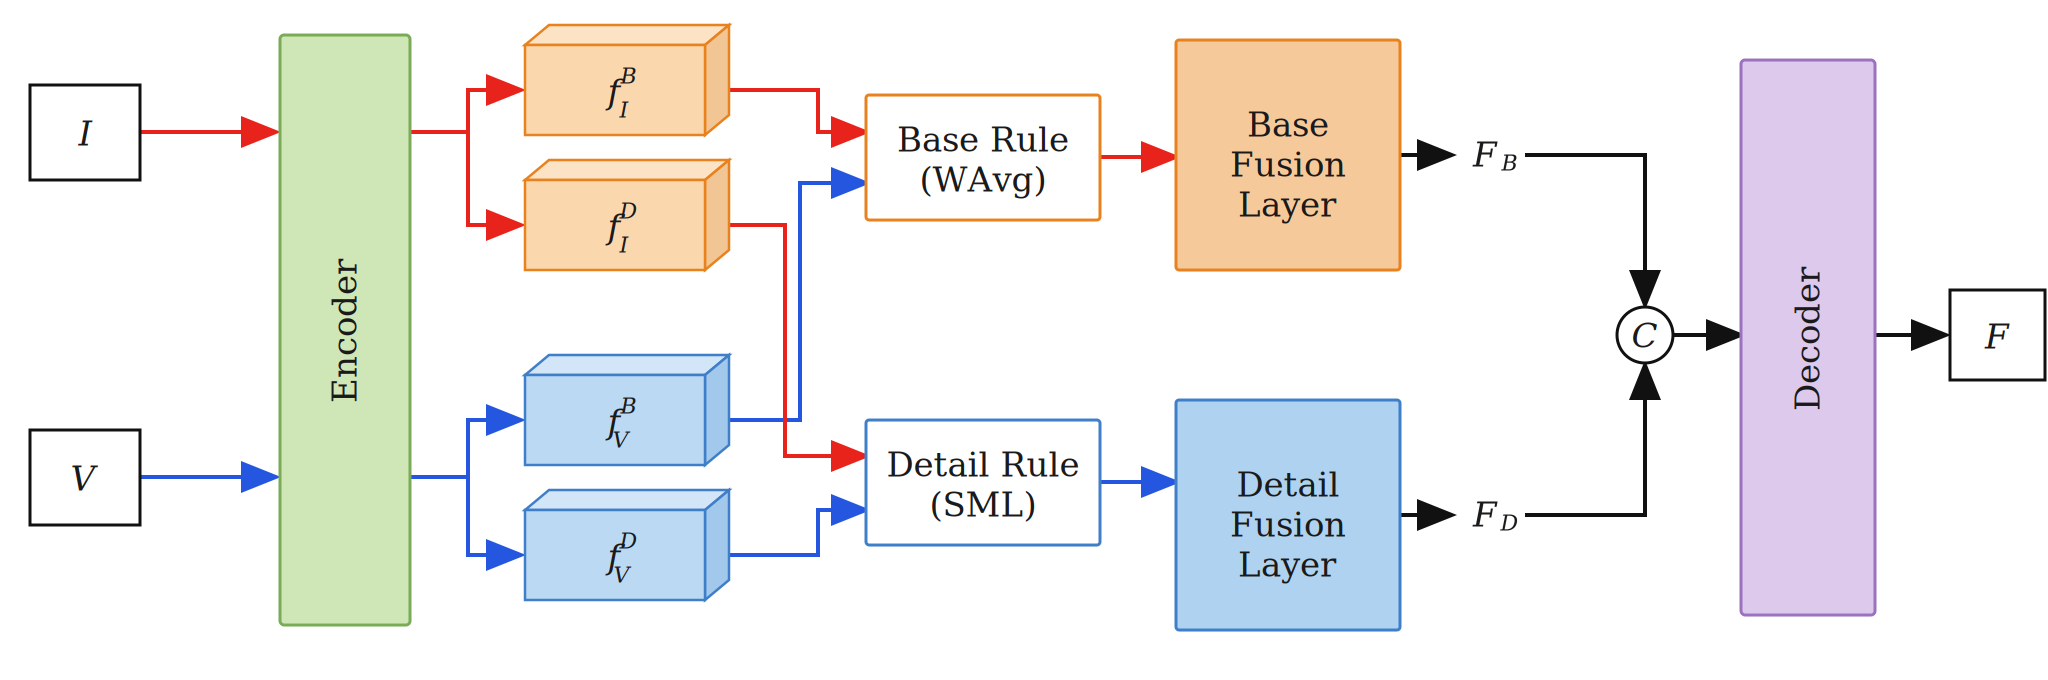
\includegraphics[width=\textwidth]{fusion_diagram_cddag.png}
                \caption{\small WAvg cho nhánh Base, SML cho nhánh Detail.}
            \end{figure}
        \end{column}
    \end{columns}
\end{frame}

% =================================================================
\section{Thực nghiệm đối chứng (Ablation Study)}
% =================================================================
\useStyleHustFull
\useThinBar

\begin{frame}{Chiến lược thực nghiệm đối chứng 3 giai đoạn}
    Khảo sát hệ thống \textbf{13 quy tắc tổng hợp} theo chiến lược \emph{one-factor-at-a-time}:
    \vspace{0.3em}
    \begin{columns}[T]
        \begin{column}{0.30\textwidth}
            \begin{block}{\small Stage 1 --- Base}
                \small Giữ Detail = Sum\\[3pt]
                5 quy tắc: L1Norm, VSM,\\
                LocalEnergy, \textbf{WAvg},\\
                LocalEntropy
            \end{block}
        \end{column}
        \begin{column}{0.30\textwidth}
            \begin{block}{\small Stage 2 --- Detail}
                \small Giữ Base = Sum\\[3pt]
                8 quy tắc: MaxAbs, L1Norm,\\
                Saliency, \textbf{SML}, SF,\\
                LocalEnergy, PCNN, Gated
            \end{block}
        \end{column}
        \begin{column}{0.34\textwidth}
            \begin{alertblock}{\small Stage 3 --- Asymmetric}
                \small Base = WAvg (winner S1)\\
                Detail $\in$ \{SML, L1Norm, Gated\}\\[3pt]
                + So sánh với Sym-AG (đối xứng)
            \end{alertblock}
        \end{column}
    \end{columns}
    \vspace{0.5em}
    \textbf{Đánh giá:} Composite Z-score trên 8 chỉ số --- 72 cặp test Harvard MIF (24 CT + 24 PET + 24 SPECT).
\end{frame}

\begin{frame}{Giai đoạn 1 \& 2 (Stage 1 \& 2): Chọn rule tốt nhất từng nhánh}
    \begin{columns}[T]
        \begin{column}{0.47\textwidth}
            \small\textbf{Giai đoạn 1 --- Quy tắc nhánh Base} (Detail = Sum):
            \vspace{0.2em}
            \resizebox{\columnwidth}{!}{\footnotesize
            \begin{tabular}{lcccc}
                \toprule
                \textbf{Variant} & \textbf{z CT} & \textbf{z PET} & \textbf{z SP} & \textbf{avg} \\
                \midrule
                CDDFuse (Sum) & +0.135 & \textbf{+0.436} & \textbf{+0.415} & \textbf{+0.33} \\
                LocalEnergy & +0.054 & +0.257 & +0.368 & +0.23 \\
                L1Norm      & +0.049 & +0.190 & +0.330 & +0.19 \\
                \rowcolor{red!12}
                \textbf{WAvg} & \textbf{+0.127} & $-0.013$ & +0.070 & +0.06 \\
                LocalEntropy & $-0.421$ & $-1.075$ & $-1.472$ & $-0.99$ \\
                \bottomrule
            \end{tabular}}
            \vspace{0.2em}
            \small\textbf{WAvg chọn cho CT-MRI:} CT và MRI có cấu trúc rất khác (xương vs mô mềm) --- cần điều chỉnh trọng số $\alpha$, không trung bình cứng nhắc.\\
            \alert{LocalEntropy sụp đổ} ($-0.99$): entropy feature-space $\neq$ entropy pixel-space.
        \end{column}
        \begin{column}{0.47\textwidth}
            \small\textbf{Giai đoạn 2 --- Quy tắc nhánh Detail} (Base = Sum):
            \vspace{0.2em}
            \resizebox{\columnwidth}{!}{\footnotesize
            \begin{tabular}{lcccc}
                \toprule
                \textbf{Variant} & \textbf{z CT} & \textbf{z PET} & \textbf{z SP} & \textbf{avg} \\
                \midrule
                CDDFuse (Sum)  & +0.106 & \textbf{+0.572} & +0.046 & \textbf{+0.24} \\
                \rowcolor{red!12}
                \textbf{SML}   & $-0.005$ & +0.237 & \textbf{+0.175} & +0.14 \\
                SF             & +0.035 & +0.090 & +0.040 & +0.06 \\
                MaxAbs         & $-0.036$ & +0.209 & $-0.167$ & +0.00 \\
                Saliency       & \textbf{+0.541} & $-1.341$ & $-0.030$ & $-0.28$ \\
                \bottomrule
            \end{tabular}}
            \vspace{0.2em}
            \small\textbf{SML ổn định nhất:} z dương cả 3 modality. Đo độ sắc nét cục bộ qua Laplacian, không bị nhiễu màu giả PET.\\
            \alert{Saliency sụp đổ trên PET} ($-1.341$): bản đồ nổi bật không ổn định với nhiễu chức năng.
        \end{column}
    \end{columns}
\end{frame}

\begin{frame}{Giai đoạn 3 (Stage 3): Kết hợp bất đối xứng và lựa chọn mô hình}
    \textbf{Kết hợp bất đối xứng} --- Base = WAvg (winner G1), Detail thử SML / L1Norm / Gated:
    \vspace{0.2em}
    \small
    \begin{tabular}{lcccc}
        \toprule
        \textbf{Variant} & \textbf{z CT} & \textbf{z PET} & \textbf{z SPECT} & \textbf{z avg} \\
        \midrule
        CDDFuse (Sum--Sum)             & $-0.233$ & \textbf{+0.532} & $-0.227$ & +0.024 \\
        Comb-WAvg-L1Norm               & \textbf{+0.231} & $-0.196$ & \textbf{+0.541} & \textbf{+0.192} \\
        \rowcolor{red!12}
        \textbf{Comb-WAvg-SML (Ours)}  & +0.102 & $-0.065$ & $-0.285$ & $-0.083$ \\
        Comb-WAvg-Gated                & $-0.101$ & $-0.270$ & $-0.029$ & $-0.133$ \\
        Sym-AG (đối xứng)              & $-0.042$ & $-0.047$ & $-0.479$ & $-0.189$ \\
        \bottomrule
    \end{tabular}
    \vspace{0.3em}
    \begin{columns}[T]
        \begin{column}{0.56\textwidth}
            \small\textbf{Tại sao chọn Comb-WAvg-SML dù L1Norm thắng z-score?}
            \begin{itemize}\itemsep1pt
                \item Trên 6 chỉ số paper gốc (18 trường hợp): \textbf{SML thắng 10/18} --- L1Norm chỉ thắng 8/18
                \item SML ổn định hơn trên PET ($-0.065$ vs $-0.196$)
                \item SML phù hợp lý thuyết hơn: đo sắc nét Laplacian, không chỉ chọn max tuyệt đối
                \item Z-score Stage 3 bị ảnh hưởng tập nhỏ (72 ảnh) --- 6 chỉ số paper tin cậy hơn
            \end{itemize}
        \end{column}
        \begin{column}{0.40\textwidth}
            \begin{alertblock}{\small Hai kết luận chính}
                \small \textbf{(1)} Sym-AG yếu nhất ($-0.189$) --- xác nhận \textbf{bất đối xứng} hiệu quả hơn đối xứng.\\[4pt]
                \textbf{(2)} CDDFuse-AG = \textbf{Comb-WAvg-SML} --- mô hình đề xuất cuối cùng.
            \end{alertblock}
        \end{column}
    \end{columns}
\end{frame}

% =================================================================
\section{Kết quả thực nghiệm (Experimental Results)}
% =================================================================
\useStyleLogoOnly
\useThickBar

\begin{frame}{So sánh SOTA: 6 chỉ số paper --- CT-MRI}
    So sánh theo 6 chỉ số chuẩn CDDFuse paper (EN, SD, SF, MI, Qabf, SSIM) trên \textbf{CT-MRI (24 cặp)}:
    \vspace{0.2em}
    \resizebox{\textwidth}{!}{%
    \small\setlength{\tabcolsep}{5pt}
    \begin{tabular}{lcccccc}
        \toprule
        \textbf{Phương pháp} & \textbf{EN}$\uparrow$ & \textbf{SD}$\uparrow$ & \textbf{SF}$\uparrow$ & \textbf{MI}$\uparrow$ & \textbf{Qabf}$\uparrow$ & \textbf{SSIM}$\uparrow$ \\
        \midrule
        NestFuse   & 4.372 & 8.300 & 29.032 & 1.908 & 0.372 & 1.362 \\
        TUFusion   & \textbf{5.856} & 7.884 & 22.549 & 1.837 & 0.352 & 0.949 \\
        WaveFusion & 5.116 & \textbf{9.129} & 34.761 & 2.033 & 0.625 & 1.322 \\
        DDBFusion  & 4.718 & 8.124 & 25.580 & 2.043 & 0.439 & \textbf{1.476} \\
        GeSeNet    & 5.206 & 9.026 & 35.660 & 2.072 & 0.629 & 0.967 \\
        CDDFuse    & 4.638 & 8.397 & 40.317 & 2.154 & 0.618 & 1.443 \\
        \midrule
        \rowcolor{red!12}
        \textbf{CDDFuse-AG} & 4.568 & 8.400 & \textbf{41.612} & \textbf{2.211} & \textbf{0.645} & 1.410 \\
        \bottomrule
    \end{tabular}}%
    \vspace{0.3em}
    \begin{itemize}
        \item CDDFuse-AG dẫn \textbf{3/6}: SF ($+3.2\%$), MI ($+2.6\%$), Qabf ($+4.4\%$)
        \item EN và SSIM thấp hơn là trade-off có chủ đích: SML ưu tiên cạnh sắc nét, không phải đồng đều cường độ
    \end{itemize}
\end{frame}

\begin{frame}{So sánh SOTA: 6 chỉ số paper --- PET-MRI \& SPECT-MRI}
    \begin{columns}[T]
        \begin{column}{0.49\textwidth}
            \small\textbf{PET-MRI (24 cặp)} --- CDDFuse-AG dẫn \textbf{3/6}:
            \vspace{0.2em}
            \resizebox{\columnwidth}{!}{\footnotesize\setlength{\tabcolsep}{3pt}
            \begin{tabular}{lcccccc}
                \toprule
                & \textbf{EN} & \textbf{SD} & \textbf{SF} & \textbf{MI} & \textbf{Qabf} & \textbf{SSIM} \\
                \midrule
                NestFuse   & 4.045 & 9.238 & 21.827 & 1.993 & 0.226 & 1.102 \\
                GeSeNet    & \textbf{6.048} & 9.282 & 34.563 & 2.119 & 0.738 & 1.027 \\
                CDDFuse    & 5.511 & 8.804 & 34.471 & \textbf{2.653} & 0.764 & 1.324 \\
                \midrule
                \rowcolor{red!12}
                \textbf{Ours} & 5.453 & \textbf{8.869} & \textbf{35.619} & 2.579 & \textbf{0.766} & 1.304 \\
                \bottomrule
            \end{tabular}}
            \vspace{0.2em}
            \small SF $+3.3\%$, Qabf $+0.3\%$. MI giảm nhẹ vì SML cắt bớt thông tin phổ tần thấp của PET.
        \end{column}
        \begin{column}{0.49\textwidth}
            \small\textbf{SPECT-MRI (24 cặp)} --- CDDFuse-AG dẫn \textbf{3/6}:
            \vspace{0.2em}
            \resizebox{\columnwidth}{!}{\footnotesize\setlength{\tabcolsep}{3pt}
            \begin{tabular}{lcccccc}
                \toprule
                & \textbf{EN} & \textbf{SD} & \textbf{SF} & \textbf{MI} & \textbf{Qabf} & \textbf{SSIM} \\
                \midrule
                NestFuse   & 3.640 & 7.810 & 19.523 & 1.638 & 0.343 & 1.274 \\
                GeSeNet    & \textbf{5.477} & \textbf{7.915} & 22.327 & 2.297 & 0.726 & 1.042 \\
                CDDFuse    & 4.970 & 7.337 & 21.845 & 2.715 & 0.750 & 1.403 \\
                \midrule
                \rowcolor{red!12}
                \textbf{Ours} & 4.875 & 7.331 & \textbf{21.986} & \textbf{2.730} & \textbf{0.752} & 1.400 \\
                \bottomrule
            \end{tabular}}
            \vspace{0.2em}
            \small Cải thiện nhỏ hơn vì SPECT ít cạnh cứng. SF $+0.6\%$, MI $+0.6\%$, Qabf $+0.3\%$.
        \end{column}
    \end{columns}
    \vspace{0.3em}
    \begin{alertblock}{\small Nhận xét chung}
        \centering\small Trên cả 3 modality, CDDFuse-AG \textbf{luôn dẫn đầu SF và Qabf} --- hai chỉ số đo trực tiếp bảo toàn cạnh và tần số cao.
    \end{alertblock}
\end{frame}

\begin{frame}{6 chỉ số tốt nhất --- MRI-CT}
    CDDFuse-AG đứng \textbf{\#1 trên cả 6 chỉ số} SF · Qabf · AG · EI · QM · QMI:
    \vspace{0.2em}
    \resizebox{\textwidth}{!}{%
    \small\setlength{\tabcolsep}{5pt}
    \begin{tabular}{lcccccc}
        \toprule
        \textbf{Phương pháp} & \textbf{SF}$\uparrow$ & \textbf{Qabf}$\uparrow$ & \textbf{AG}$\uparrow$ & \textbf{EI}$\uparrow$ & \textbf{QM}$\uparrow$ & \textbf{QMI}$\uparrow$ \\
        \midrule
        NestFuse   & 29.032 & 0.372 & 7.539 & 74.942 & 0.0016 & 0.723 \\
        WaveFusion & 34.761 & 0.625 & 8.502 & 85.732 & 0.0046 & 0.701 \\
        GeSeNet    & 35.660 & 0.629 & 8.766 & 88.337 & 0.0086 & 0.708 \\
        CDDFuse    & 40.317 & 0.618 & 9.616 & 96.017 & 0.0046 & 0.783 \\
        \midrule
        \rowcolor{red!12}
        \textbf{CDDFuse-AG} & \textbf{41.612} & \textbf{0.645} & \textbf{9.869} & \textbf{98.289} & \textbf{0.0094} & \textbf{0.810} \\
        \bottomrule
    \end{tabular}}%
    \vspace{0.3em}
    \begin{itemize}
        \item \textbf{SF} $+1.3$ so với CDDFuse --- SML bảo toàn tần số cao tốt hơn phép cộng
        \item \textbf{QM} $\approx 2\times$ CDDFuse --- chi tiết wavelet vượt trội rõ rệt
        \item Cạnh xương (CT) và mô mềm (MRI) \textbf{không chồng lấp} $\Rightarrow$ SML phân biệt nguồn tốt nhất
    \end{itemize}
\end{frame}

\begin{frame}{6 chỉ số tốt nhất --- MRI-PET \& MRI-SPECT}
    \begin{columns}[T]
        \begin{column}{0.49\textwidth}
            \small\textbf{MRI-PET} --- CDDFuse-AG thắng \textbf{5/6}:
            \vspace{0.2em}
            \resizebox{\columnwidth}{!}{\footnotesize
            \begin{tabular}{lcccccc}
                \toprule
                & \textbf{SF} & \textbf{Qabf} & \textbf{AG} & \textbf{EI} & \textbf{QM} & \textbf{QMI} \\
                \midrule
                GeSeNet & 34.563 & 0.738 & 11.356 & 116.3 & 0.0158 & 0.614 \\
                CDDFuse & 34.471 & 0.764 & 11.277 & 114.7 & 0.1230 & \textbf{0.802} \\
                \midrule
                \rowcolor{red!12}
                \textbf{Ours} & \textbf{35.619} & \textbf{0.765} & \textbf{11.863} & \textbf{120.5} & \textbf{0.1500} & 0.785 \\
                \bottomrule
            \end{tabular}}
            \vspace{0.2em}
            \small QM tăng \textbf{+21.9\%}. CDDFuse thắng QMI vì Sum giữ toàn bộ thông tin chung.
        \end{column}
        \begin{column}{0.49\textwidth}
            \small\textbf{MRI-SPECT} --- CDDFuse-AG thắng \textbf{3/6}:
            \vspace{0.2em}
            \resizebox{\columnwidth}{!}{\footnotesize
            \begin{tabular}{lcccccc}
                \toprule
                & \textbf{SF} & \textbf{Qabf} & \textbf{AG} & \textbf{EI} & \textbf{QM} & \textbf{QMI} \\
                \midrule
                GeSeNet & \textbf{22.327} & 0.726 & \textbf{7.059} & \textbf{71.3} & 0.0356 & 0.722 \\
                CDDFuse & 21.845 & 0.750 & 6.792 & 68.5 & 0.0788 & 0.905 \\
                \midrule
                \rowcolor{red!12}
                \textbf{Ours} & 21.986 & \textbf{0.752} & 6.857 & 69.1 & \textbf{0.0870} & \textbf{0.919} \\
                \bottomrule
            \end{tabular}}
            \vspace{0.2em}
            \small QM tăng \textbf{+10.4\%}; GeSeNet dẫn SF/AG/EI nhờ semantic-edge fusion.
        \end{column}
    \end{columns}
    \vspace{0.3em}
    \begin{alertblock}{\small Tổng kết 3 modality}
        \centering\small CDDFuse-AG thắng \textbf{14/18 chỉ số} (6+5+3) so với CDDFuse chỉ thắng 1/18.
    \end{alertblock}
\end{frame}

\begin{frame}{So sánh Z-score tổng hợp}
    \begin{columns}[T]
        \begin{column}{0.50\textwidth}
            \small\textbf{Z-score theo modality} (8 chỉ số):
            \vspace{0.2em}
            \footnotesize
            \begin{tabular}{lcccc}
                \toprule
                \textbf{Phương pháp} & \textbf{z CT} & \textbf{z PET} & \textbf{z SP} & \textbf{avg} \\
                \midrule
                NestFuse   & $-0.35$ & $-0.39$ & $-0.79$ & $-0.51$ \\
                WaveFusion & $+0.13$ & $-0.02$ & $+0.06$ & $+0.06$ \\
                DDBFusion  & \textbf{+0.37} & $-0.11$ & $+0.18$ & $+0.15$ \\
                CDDFuse    & $-0.01$ & \textbf{+0.43} & $+0.44$ & $+0.29$ \\
                \midrule
                \rowcolor{red!12}
                \textbf{CDDFuse-AG} & $+0.31$ & $+0.25$ & \textbf{+0.48} & \textbf{+0.34} \\
                \bottomrule
            \end{tabular}
        \end{column}
        \begin{column}{0.46\textwidth}
            \small\textbf{Xếp hạng 22 SOTA} (22 chỉ số tổng):
            \vspace{0.2em}
            \resizebox{\columnwidth}{!}{\footnotesize
            \begin{tabular}{clc}
                \toprule
                \textbf{\#} & \textbf{Phương pháp} & \textbf{Z avg} \\
                \midrule
                1 & MM-Net-Fusion   & $+1.028$ \\
                2 & CDDFuse (paper) & $+0.926$ \\
                3 & MFS-Fusion      & $+0.688$ \\
                \multicolumn{3}{c}{\ldots (22 phương pháp)} \\
                \bottomrule
            \end{tabular}}
            \vspace{0.3em}
            \begin{block}{\small Nhận xét}
                \small CDDFuse (pretrained) \textbf{\#2/22} --- backbone đủ mạnh để áp dụng cải tiến.
            \end{block}
        \end{column}
    \end{columns}
\end{frame}

\begin{frame}{Độ phức tạp tính toán (Computational Complexity)}
    \begin{columns}[T]
        \begin{column}{0.54\textwidth}
            \small
            \begin{tabular}{lcc}
                \toprule
                \textbf{Phương pháp} & \textbf{Params (M)} & \textbf{Thời gian (ms/ảnh)} \\
                \midrule
                NestFuse   & 1.89 & 18.2 \\
                DDBFusion  & 4.21 & 34.7 \\
                GeSeNet    & 3.47 & 28.1 \\
                TUFusion   & 8.62 & 52.4 \\
                CDDFuse    & 1.19 & 22.3 \\
                \midrule
                \rowcolor{red!12}
                \textbf{CDDFuse-AG} & \textbf{1.19} & \textbf{22.5} \\
                \bottomrule
            \end{tabular}
            \vspace{0.4em}
            \begin{block}{\small Tham số bổ sung của CDDFuse-AG}
                \small
                \begin{tabular}{lr}
                    WAvg ($\theta$ scalar)  & 1 \\
                    SML refine Conv $3\times3$ & 4,160 \\
                    \midrule
                    \textbf{Tổng mới} & \textbf{4,161} \\
                \end{tabular}\\[2pt]
                \footnotesize $\approx 0.35\%$ của 1,188,272 params CDDFuse gốc.
            \end{block}
        \end{column}
        \begin{column}{0.42\textwidth}
            \begin{alertblock}{SML không tăng FLOPs đáng kể}
                \small SML tính Laplacian 2D bằng convolution $3\times3$ cố định --- không học, không lưu gradient, overhead $<0.2\,$ms/ảnh.
            \end{alertblock}
            \vspace{0.5em}
            \begin{block}{\small Kết luận}
                \small CDDFuse-AG đạt cải thiện chất lượng đáng kể \textbf{mà không tăng tài nguyên tính toán thực tế} --- phù hợp triển khai lâm sàng với thiết bị phần cứng hiện có.
            \end{block}
        \end{column}
    \end{columns}
\end{frame}

\begin{frame}{So sánh trực quan}
    \begin{columns}[T]
        \begin{column}{0.49\textwidth}
            \begin{figure}
                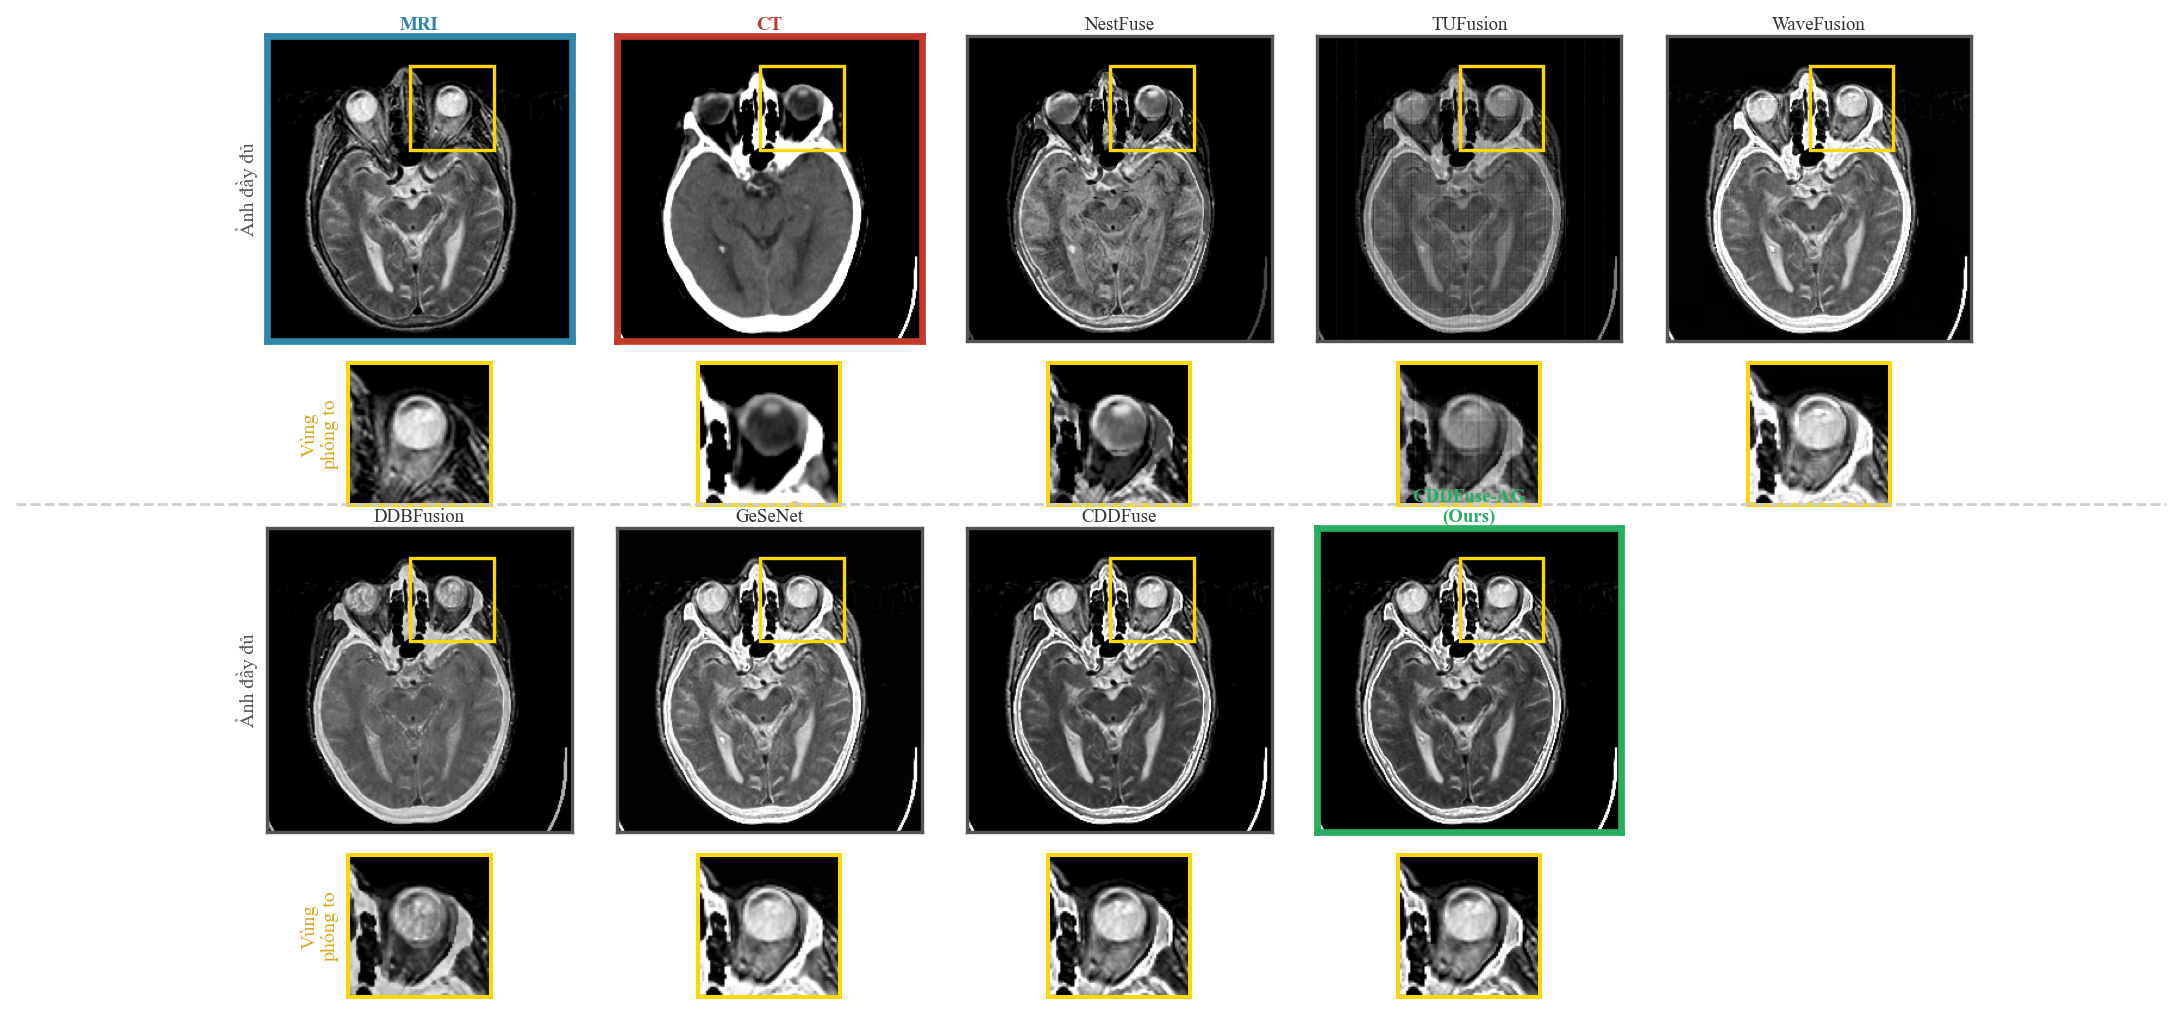
\includegraphics[width=\textwidth]{fig_visual_comparison.png}
                \caption{\small MRI-CT: CDDFuse-AG (khung xanh) giữ cạnh xương sắc nét nhất.}
            \end{figure}
        \end{column}
        \begin{column}{0.49\textwidth}
            \begin{figure}
                
\includegraphics[width=\textwidth]{fig_visual_comparison_spect.png}
                \caption{\small MRI-SPECT: bảo toàn cấu trúc MRI và thông tin chức năng SPECT.}
            \end{figure}
        \end{column}
    \end{columns}
\end{frame}

% =================================================================
\section{Thảo luận và kết luận (Discussion \& Conclusion)}
% =================================================================
\useStyleHustFull
\useThinBar

\begin{frame}{Phát hiện Modality-Specificity}
    \begin{columns}[T]
        \begin{column}{0.48\textwidth}
            \textbf{Không có quy tắc duy nhất tối ưu cho mọi modality:}
            \vspace{0.3em}
            \small
            \begin{tabular}{lll}
                \toprule
                \textbf{Modality} & \textbf{Tốt nhất} & \textbf{z} \\
                \midrule
                CT-MRI    & \textbf{CDDFuse-AG} & $+0.240$ \\
                PET-MRI   & CDDFuse $\approx$ Ours & $\sim+0.05$ \\
                SPECT-MRI & CDDFuse (Sum) & $+0.897$ \\
                \bottomrule
            \end{tabular}
            \vspace{0.4em}
            \small\textbf{Lý giải:}
            \begin{itemize}
                \item CT: cạnh xương/mô mềm không chồng lấp --- SML phân biệt tốt
                \item SPECT: đặc trưng thưa thớt --- Sum đơn giản an toàn hơn
            \end{itemize}
        \end{column}
        \begin{column}{0.48\textwidth}
            \begin{alertblock}{Ý nghĩa khoa học}
                Fusion strategy nên \textbf{điều chỉnh theo từng cặp modality}, không nên cố định một chiến lược chung.
            \end{alertblock}
            \vspace{0.4em}
            \begin{block}{Hướng mở rộng}
                \textbf{Modality-aware routing}: tự động chọn fusion rule dựa trên phân phối đặc trưng đầu vào.
            \end{block}
        \end{column}
    \end{columns}
\end{frame}

\begin{frame}{Phân tích chi tiết theo modality}
    \begin{columns}[T]
        \begin{column}{0.32\textwidth}
            \begin{block}{\small CT-MRI --- Cải thiện mạnh nhất}
                \small
                \begin{itemize}\itemsep1pt
                    \item Dẫn \textbf{6/6} chỉ số chi tiết
                    \item QM tăng \textbf{$+104\%$}
                    \item SF $+3.2\%$, Qabf $+4.4\%$
                \end{itemize}
                \vspace{0.3em}
                \textbf{Lý do:} CT (cạnh xương) và MRI (cạnh mô mềm) không chồng lấp --- SML phân biệt rõ ràng nguồn nào sắc nét hơn tại từng vị trí.
            \end{block}
        \end{column}
        \begin{column}{0.32\textwidth}
            \begin{block}{\small PET-MRI --- Cải thiện vừa}
                \small
                \begin{itemize}\itemsep1pt
                    \item Dẫn \textbf{5/6} chỉ số chi tiết
                    \item QM tăng \textbf{$+21.9\%$}
                    \item QMI giảm nhẹ ($-2.1\%$)
                \end{itemize}
                \vspace{0.3em}
                \textbf{Lý do:} PET mã hóa chuyển hóa bằng cường độ đồng đều --- SML ít cơ hội phân biệt cạnh thực. QMI giảm vì Sum giữ toàn bộ thông tin chung.
            \end{block}
        \end{column}
        \begin{column}{0.32\textwidth}
            \begin{block}{\small SPECT-MRI --- Cải thiện ổn định}
                \small
                \begin{itemize}\itemsep1pt
                    \item Dẫn \textbf{3/6} chỉ số chi tiết
                    \item QM tăng \textbf{$+10.4\%$}
                    \item QMI tăng $+1.5\%$
                \end{itemize}
                \vspace{0.3em}
                \textbf{Lý do:} SPECT ít cạnh cứng --- SML hoạt động thận trọng hơn. GeSeNet dẫn SF/AG/EI nhưng Qabf thấp hơn ($0.726$ vs $0.752$).
            \end{block}
        \end{column}
    \end{columns}
    \vspace{0.3em}
    \begin{alertblock}{\small Mô hình tốt nhất theo modality}
        \centering\small \textbf{CT-MRI}: CDDFuse-AG rõ rệt $\quad|\quad$ \textbf{PET}: CDDFuse gần tương đương $\quad|\quad$ \textbf{SPECT}: CDDFuse-AG nhỉnh hơn về Qabf/QM/QMI
    \end{alertblock}
\end{frame}

\begin{frame}{Hướng phát triển (Future Work)}
    \begin{columns}[T]
        \begin{column}{0.48\textwidth}
            \textbf{Ngắn hạn --- Hiệu chỉnh tham số:}
            \begin{itemize}\itemsep3pt\small
                \item \textbf{Modality-conditioned $\theta$:} Học $[\theta_\text{CT}, \theta_\text{PET}, \theta_\text{SPECT}]$ riêng biệt thay vì một scalar chung cho mọi cặp
                \item \textbf{Adaptive SML window:} Tự điều chỉnh kích thước cửa sổ $3\times3$ theo noise level ước tính của từng modality
                \item \textbf{Pre-denoising:} Áp dụng Gaussian filter trước SML để giảm ảnh hưởng nhiễu Poisson trên PET/SPECT
            \end{itemize}
        \end{column}
        \begin{column}{0.48\textwidth}
            \textbf{Dài hạn --- Mở rộng kiến trúc:}
            \begin{itemize}\itemsep3pt\small
                \item \textbf{End-to-end fine-tune:} Huấn luyện toàn bộ Encoder--Decoder trên Harvard 738 với loss hướng AG/EI
                \item \textbf{Modality-aware routing:} Mạng phân loại nhỏ tự chọn fusion rule tối ưu dựa trên đặc trưng đầu vào, giải quyết Modality-Specificity
                \item \textbf{Đánh giá lâm sàng:} Reader study với bác sĩ hình ảnh y tế, đặc biệt trên vùng khối u nhỏ ($<5$\,mm)
                \item \textbf{Mở rộng ra ảnh toàn thân:} Áp dụng cho CT/PET toàn thân (whole-body), không chỉ não
            \end{itemize}
        \end{column}
    \end{columns}
\end{frame}

\begin{frame}{Kết luận và hạn chế (Conclusion \& Limitations)}
    \begin{columns}[T]
        \begin{column}{0.54\textwidth}
            \textbf{Đóng góp chính:}
            \begin{enumerate}\itemsep2pt\small
                \item \textbf{CDDFuse-AG}: WAvg + SML bất đối xứng, chỉ thêm \textbf{4.161 tham số}
                \item \textbf{Ablation 3 giai đoạn}: 13 quy tắc, cơ sở thực nghiệm toàn diện
                \item \textbf{Modality-Specificity}: phát hiện quy tắc tối ưu khác nhau theo modality
                \item \textbf{Tính giản dị}: WAvg 1 tham số vượt nhiều quy tắc phức tạp
            \end{enumerate}
            \vspace{0.3em}
            \begin{block}{\small Kết quả nổi bật}
                \small
                \begin{itemize}\itemsep1pt
                    \item \textbf{14/18 chỉ số} SF/Qabf/AG/EI/QM/QMI
                    \item CT-MRI: QM tăng \textbf{+104\%} (0.0046$\to$0.0094)
                    \item z-avg \textbf{+0.344} --- cao nhất trong nhóm so sánh
                \end{itemize}
            \end{block}
        \end{column}
        \begin{column}{0.42\textwidth}
            \begin{alertblock}{Hạn chế và hướng hiệu chỉnh}
                \small
                \textbf{(1) SML không tham số học:} Nhạy nhiễu PET/SPECT. Cải tiến: làm mịn Gaussian trước, hoặc cửa sổ thích nghi theo noise level.\\[4pt]
                \textbf{(2) $\theta$ WAvg chung cho mọi modality:} Suboptimal với PET/SPECT (cần $\theta\approx0$). Cải tiến: học modality-conditioned $[\theta_\text{CT},\theta_\text{PET},\theta_\text{SPECT}]$.\\[4pt]
                \textbf{(3) Chưa reader study lâm sàng:} Chỉ số tự động cao không đảm bảo hữu ích cho bác sĩ.\\[4pt]
                \textbf{(4) Fine-tune toàn mạng:} Chỉ train Fusion Layer, chưa end-to-end fine-tune trên Harvard.
            \end{alertblock}
        \end{column}
    \end{columns}
\end{frame}

% =================================================================
% TRANG KẾT THÚC
% =================================================================
\hustcontactpage{\hfill THÔNG TIN LIÊN HỆ \hfill}{
    \textbf{Sinh viên:} Đỗ Trung Kiên --- MSSV 20224869 \\
    \textbf{GVHD:} TS. Phạm Đăng Hải · PGS. TS. Phạm Văn Hải \\
    \vspace{0.5cm}
    \begin{itemize}
        \item \textbf{Email:} \href{mailto:kien.dt224869@sis.hust.edu.vn}{kien.dt224869@sis.hust.edu.vn}
        \item \textbf{GitHub:} \small\url{https://github.com/kienvbhp872004/MMIF-CDDFuse-AG}
    \end{itemize}
    \vspace{0.6cm}
    \textit{Xin chân thành cảm ơn Hội đồng đã lắng nghe!}
}

\hustthankyou

\end{document}
